\documentclass{easychair}

% \usepackage{doc}
\usepackage{setspace}
\usepackage{verbatim}
\usepackage{amssymb}

%----Making things more compact
\newcommand{\smalltt}[1]{\small \texttt{#1}}
\newenvironment{packed_itemize}{
\vspace*{-0.2em}
\begin{itemize}
\setlength{\partopsep}{0pt}
\setlength{\itemsep}{1pt}
\setlength{\parskip}{0pt}
\setlength{\parsep}{0pt}
}{\end{itemize}}
\newenvironment{packed_enumerate}{
\vspace*{-0.2em}
\begin{enumerate}
\setlength{\partopsep}{0pt}
\setlength{\itemsep}{1pt}
\setlength{\parskip}{0pt}
\setlength{\parsep}{0pt}
}{\end{enumerate}}
% \renewcommand{\textfraction}{0.07}
% \renewcommand{\topfraction}{0.9}
% \renewcommand{\bottomfraction}{0.9}
% \renewcommand{\floatpagefraction}{0.66}
% \setlength{\floatsep}{2.0pt plus 2.0pt minus 2.0pt}
% \setlength{\textfloatsep}{5.0pt plus 2.0pt minus 0.0pt}

\title{The New TPTP Format for \\ Tarskian and Kripke Interpretations}

\author{
  Geoff Sutcliffe\inst{1}
\and
  Alexander Steen\inst{2}
\and
  Pascal Fontaine\inst{3}
}

\institute{
  University of Miami,
  Miami, USA\\
  \email{geoff@cs.miami.edu,jam771@miami.edu}
\and
  University of Greifswald,
  Greifswald, Germany\\
  \email{alexander.steen@uni-greifswald.de}
\and
  University of Li{\`e}ge,
  Li{\`e}ge, Belgium\\
  \email{Pascal.Fontaine@uliege.be}
}

\authorrunning{Sutcliffe, Steen, Fontaine}
\titlerunning{TPTP World Interpretations}

\begin{document}
\maketitle

%--------------------------------------------------------------------------------------------------
\begin{abstract}
This paper describes a new format for representing Tarskian and Kripke interpretations.
%formulae in untyped and typed first-order logic, using the TPTP TF0 language.
\end{abstract}
%--------------------------------------------------------------------------------------------------
\section{Introduction}
\label{Introduction}

Historically, Automated Theorem Proving (ATP) has, as the name suggests, focused largely on the
task of proving theorems from axioms -- the derivation of conclusions that follow inevitably 
from known facts \cite{RV01-HAR}.
The axioms and conjecture to be proved (and hence become a theorem) are written in an 
appropriately expressive logic, and the proofs are often similarly written in logic \cite{SS+06}.
In the last two decades the converse task of disproving conjectures, i.e., proving that a 
conjecture is not a theorem of the axioms, has become increasingly important.
This process depends on finding an {\em interpretation}, i.e., a structure that maps terms 
to domain elements and formulae to truth values.
An interpretation that maps a formula to {\em true} is a {\em model} of the formula.
A conjecture is disproved by finding an interpretation that is a model of the axioms, but 
is not a model of the conjecture, aka a {\em countermodel} for the conjecture.
A salient application area that harnesses this form of ATP is verification \cite{DKW08},
where a countermodel is used to pinpoint the reason why a proof obligation fails, and
correspondingly points to the location of the fault in the system being verified.
Other applications of model finding include checking the consistency of an axiomatization 
\cite{SS+17}, and finding a solution to a problem that is coded as a model finding problem 
\cite{Win82}.

The TPTP World \cite{Sut17} (\href{https://www.tptp.org}{\tt www.tptp.org}) is a well established 
infrastructure that supports research, development, and deployment of 
% Automated Theorem Proving 
ATP systems.
Various parts of the TPTP World have been deployed in a range of applications, in both academia 
and industry.
The TPTP World includes the TPTP problem library \cite{Sut09}, 
the TSTP solution library \cite{Sut10}, 
tools and services for processing ATP problems and solutions \cite{Sut10}, 
it supports the CADE ATP System Competition (CASC) \cite{Sut16}.
The TPTP language \cite{Sut23-IGPL} is one of the keys to the success of the TPTP World.
Originally the TPTP World supported only first-order clause normal form (CNF)
\cite{SS98-JAR}.
Over the years full first-order form (FOF)
\cite{Sut09}, 
typed first-order form (TFF)
\cite{SS+12,BP13-TFF1}, 
typed extended first-order form (TXF)
\cite{SK18}, 
typed higher-order form (THF)
\cite{SB10,KSR16}, 
and non-classical forms (NTF).
Most relevant to this work, the TPTP languages are used for writing ATP problems, 
derivations, and interpretations \cite{SS+06,Sut08-KEAPPA}.
Examples of problems are in Appendices~\ref{FOF_Finite.p}, \ref{TFF_Finite.p},
\ref{TFF_Infinite.p}, \ref{THF_Finite.p}, \ref{NTF_Finite-Finite-Global.p}, 
and~\ref{NTF_Finite-Finite-Local.p}.

A TPTP format for interpretations with finite domains \cite{SS+06} was previously been defined, 
and has served the ATP community adequately for almost 20 years. 
The old format is output by several ATP systems, e.g., Paradox \cite{CS03}, FMDarwin \cite{BF+06}, 
Vampire \cite{KV13}.
Recently the need for a format for interpretations with infinite domains, and for a format for 
Kripke interpretations \cite{Kri63} of formulae written in the NTF language \cite{SF+22}, 
led to the development of a new TPTP format for interpretations.
This work describes the new TPTP format for interpretations.
The underlying principle is unchanged: interpretations are represented as formulae.

\paragraph{Related Work:}
There are other concrete representations of interpretations in use:
The SMT-LIB standard \cite{BFT17} defines a format for model output, and commands to inspect 
models.  
SAT solvers generally output models as specified by the SAT competitions \cite{JL+12}, in a 
simple format similar to the DIMACS input format \cite{Bab93}.
Some individual model finding systems have defined their own formats for models, e.g., the 
output formats of Nitpick and Z3 \cite{dMB08}.
% +++
% Nikolaj says ...
% Z3 It produces models that define functions by expressions. For example a model of succ is 
% Succ(x) =X+ 1
% Works when domain is integer. Currently z3 does not implement infinite models for uninterpreted sorts. I would probably support infinite sorts by creating injection into an algebraic datatype and then support models that can be expressed over ADT.
% See also https://microsoft.github.io/z3guide/docs/logic/Quantifiers
% +++

\vspace*{1em}
This paper is organized as follows:
Section~\ref{Interpretations} discusses the nature of interpretations, considering what is
needed from interpretations, and the various forms that interpretations can take.
Section~\ref{NewTarskian} defines the new format for Tarskian interpretations, and
Section~\ref{NewKripke} does the same for Kripke interpretations.
% Section~\ref{Verification} describes the semantic approach to model verification.
Section~\ref{Conclusion} concludes and discusses plans for future work.

%--------------------------------------------------------------------------------------------------
\section{About Interpretations}
\label{Interpretations}

%--------------------------------------------------------------------------------------------------
\subsection{What do we Need?}
\label{Need}

The needs of applications that require model finding vary according to their use of the model.
In the simplest case application need only to know that a model exists.
Examples of such applications include checking the consistency of an axiomatization \cite{CI15},
use as a subroutine in more complex reasoning, e.g., for
axiom selection \cite{SP07,Pud07-ESARLT}, and establishing the existence of a bug in a
verification process\footnote{%
Bill McCune claimed that establishing the existence of a bug without having an explicit model
to help pinpoint the bug would be ``frustrating''. And he should have known.}
A key weakness of model finder systems that claim to have found a model but do not output an 
explicit model is that it is necessary to trust the model finder.

In many applications it is necessary to have an explicit model, in some representation that
allows for analysis of the model.
Applications that productively use an explicit model include finding inconsistencies in 
axiomatizations \cite{SS+17}, identification of bugs in verification \cite{CE82,QS82},
solution of problems encoded as a model finding problems \cite{Win82}, and evaluating formulae
wrt the model \cite{SS+23-LPAR}.
Manual inspection of explicit models can also be useful, e.g., \cite{EK+10}.
Internally, explicit models can be used for machine learning and improving model finders.
A key advantage of having an explicit model output is that the model can be verified, i.e., the
model finder does not need to be trusted,

Given the innate desirability of obtaining explicit models of satisfiable formulae, desirable
properties of explicit models can be considered.
Verification (checking that the formulae evaluate to $true$ wrt the model), should be possible.
The process of evaluating formulae should be tractable.
Interpretations should be sufficiently comprehensible for manual inspection.

%--------------------------------------------------------------------------------------------------
\subsection{What do we Have?}
\label{Have}

A Tarskian-style interpretation \cite{TV56} of formulae in first-order logic consists of a 
non-empty domain of unequal elements for each type used in the formulae (just one domain for 
untyped logic), and interpretations of the function and predicate symbols with respect to the 
domains \cite{Hun96,Gal15}.
An overview of some ways of building and representing Tarskian interpretations is provided 
by \cite{CLP04}.
A {\em complete} interpretation can interpret all expressions that can be written in the language 
of the formulae, but a {\em partial} interpretation can interpret only (at least) the 
given formulae, e.g., \cite{BSW23}.
Three types of Tarskian interpretations are clear (and more might exist):
\begin{itemize}
\item {\em Finite interpretations} have only finite domains.
      The domain and symbol mappings can be be explicitly enumerated.
      Finite models for a set of formulae are typically produced by starting with domains of 
      size one, and incrementing the sizes until a model is found.
      At each iteration the formulae are reduced to either propositional \cite{CS03,McC03-MACE4-TR}
      or function free clause logic \cite{BF+09}, both of which are decidable logics.
      An ATP system that can decide the logic is used to find a model.
      There are several ATP systems that produce finite models, e.g., Paradox, FMDarwin, and 
      Vampire.
\item {\em Infinite interpretations} have one or more infinite domains.
      Infinite domains can be explicitly generated (e.g., terms representing Peano numbers), or 
      implicitly specified (e.g., some set of algebraic numbers, such as the integers).
      % HOW IS THIS DONE?
      There are some ATP systems that produce infinite models, e.g., cvc5 \cite{BB+22-cvc5}, Z3.
\item {\em Herbrand interpretations} \cite{Her30} have the Herbrand universe as the domain, 
      the mapping for non-boolean symbols (functions) is the ``identity'', and the mapping
      for boolean symbols (predicates) is from the Herbrand base to $\{true,false\}$.
      Every set of formulae induces its set of Herbrand models.
      A set of formulae might not be intended to represent it's models, e.g., the input to 
      an ATP system. 
      In the ATP context a set of formulae is often intended to at least confirm the existence
      of Herbrand models.
      Such sets can be the result from an ATP system applying model preserving transformations 
      on its input, or generated by an ATP system with the explicit intention of representing 
      Herbrand interpretations:
      \begin{packed_itemize}
      \item {\em Saturations} \cite{BG+01} are a fixed point for a set of clauses at which further 
            application of a complete inference system does not generate any new clauses.
            This approach is adopted in saturation-based ATP systems such as E \cite{SCV19},
            Prover9 \cite{McC-Prover9-URL}, Vampire, and Zipperposition \cite{VB+21}.
            While the domain of the Herbrand interpretations induced by a saturation is known 
            to be the Herbrand Universe, there is no explicit symbol interpretation that can be 
            used constructively by users.
      \item {\em Formulae} that are intended to represent Herbrand interpretations include
            a disjunction of implicit generalisations (DIGs) \cite{LM87}, and predicate
            definitions over the term algebra \cite{SK12}.
            iProver \cite{Kor08,SK12} is an ATP system that output the latter format.
      \end{packed_itemize}
Ways to make Herbrand interpretations:
\begin{packed_itemize}
\item Tableaux. as long as you use a proof confluent calculus, it is normally possible to 
      construct a model from a saturated branch \cite{Hah01}.
\item Hyper-tableaux. \cite{BFN96,Bau98,BFP07}
\item Ordered Semantic Hyper-linking \cite{PZ00} NEED TO READ
\item SGGS \cite{BP16}
\item Proving Infinite Satisfiability \cite{BB13}
\item Model Evolution with Equality \cite{BT03,BFT04,BT05,BPT11}
\item EQMC \cite{CP00,Pel03-EQMC}
\item Saturation \cite{Pel03-JSC}
\item RAMC \cite{CZ92,CP95,CP95-TAB}
\end{packed_itemize}

\end{itemize}

A {\em Kripke interpretation} \cite{Kri63} adds a layer of {\em worlds} over Tarskian
interpretations.
There can be a finite or infinite number of worlds.
There is an {\em accessibility relation} between the worlds, which can be subject to the
requirements of the logic being used, e.g., for modal logic {\bf M} the accessibility 
relation must be reflexive, i.e., every world can access itself.
Within each world there is a Tarskian interpretation, and there can be some interaction
between the worlds' interpretations if the terms designate globally MORE TO BE SAID.
The verifiability, tractability, and comprehensibility of Kripke interpretations varies
between individual cases.

The notions of interpretations, models, partial interpretations, finite interpretations,
Herbrand interpretations, etc., are captured in the SZS ontologies \cite{Sut08-KEAPPA}, as
updated at 
\href{https://www.tptp.org/cgi-bin/SeeTPTP?Category=Documents\&File=SZSOntology}{\tt www.tptp.org}
\href{https://www.tptp.org/cgi-bin/SeeTPTP?Category=Documents\&File=SZSOntology}{\tt /cgi-bin/SeeTPTP?Category=Documents\&File=SZSOntology}.
For this work the ontology was extended with a new value {\em Model Preserving} (MPR), defined
as ``Some interpretations are models of Ax, and
  all models of Ax are extended to a model of C, and
  all models of C are an extension of a model of Ax
  (which means that all models of C are models of Ax)''.
This is used for ATP transformations of satisfiable sets of formulae in which the models
of the set are unchanged, or changed only by adding new domain elements or mappings such
that they still model the original formulae.
Examples of such transformations are adding logical consequence of the set into the set, and
Skolemization.

%--------------------------------------------------------------------------------------------------
\subsection{Do we Have what we Need?}
\label{HaveNeed}

Section~\ref{Need} listed three needs for interpretations: 
\begin{packed_itemize}
\item Verifiability - the ability to verify a model by evaluating all the formulae it claims
      to model as $true$.
\item Tractability - the ability to evaluate a formula using some limited/reasonable amount of
      resources.
\item Comprehensibility - the extent to which the interpretation can be understood, typically
      by a human but possibly by a machine.
\end{packed_itemize}

The new TPTP format represents interpretations in formulae, written {\em interpretation-formula}
to avoid confusion -- the details are provided in Sections~\ref{NewTarskian} and~\ref{NewKripke}.
An interpretation-formula is written in an extension of the language of the formulae being 
interpreted, i.e., extending the same vocabulary as the formulae, and using the same syntax.
That immediately contributes to comprehensibility (but does not ensure it).

To interpret a formula wrt a given interpretation~\ldots
\begin{packed_itemize}
\item For a Kripke interpretation with finite worlds~\ldots
      \begin{packed_itemize}
      \item Interpret quantifiers over worlds using Kripke semantics.
      \item Interpret formulae within a world according to the following points.
      \end{packed_itemize}
\item For a Tarskian interpretation with finite domains or no quantification, and mappings for 
      symbols applied to domain elements~\ldots
      \begin{packed_itemize}
      \item Interpret quantifiers using Tarskian semantics.
      \item Interpret ground (grounded with domain elements) terms and atoms using the mappings.
      \item Interpret boolean formulae using the truth tables for connectives.
      \end{packed_itemize}
      This approach is taken internally in Vampire.
\item For interpretations represented by interpretation-formulae, theorem proving can be used.
      \begin{packed_itemize}
      \item If a formula can be proved from the interpretation-formulae then it is $true$ in the 
            interpretation represented by the interpretation-formulae.
      \item If a formula can be disproved from the interpretation-formulae then it is $false$ in 
            the interpretation represented by the interpretation-formulae.
      \item In practice, a formula might be neither proved nor disproved within reasonable 
            resource limits, so that nothing is known.
      \end{packed_itemize}
\item For Herbrand interpretations induced by formulae, theorem proving can be used~\ldots
      \begin{packed_itemize}
      \item If a formula can be proved from the formulae then it is $true$ in all the Herbrand 
            interpretations induced by the formulae.
      \item If a formula can be disproved from the formulae then it is $false$ in in all the 
            Herbrand interpretations induced by the formulae.
      \item In practice, a formula might be neither proved nor disproved within reasonable 
            resource limits, so that nothing is known.
      \end{packed_itemize}
\end{packed_itemize}
For an interpretation $I$ and formula $\Phi$, $I \vdash \Phi$ means that $\Phi$ is $true$ in $I$, 
i.e., $I$ is a model of formula $\Phi$.

Given ways to interpret a formula wrt a interpretation, models can be verified.
The TPTP World now offers the AGMV model verifier in the SystemOnTSTP \cite{Sut07-CSR} web 
interface \href{https://www.tptp.org/cgi-bin/SystemOnTSTP}{{\tt www.tptp.org/cgi-bin/SystemOnTSTP}}.
AGMV uses a trusted ATP system to prove each of the formulae in the satisfiable set $\Phi$
from the interpretation formula $\varphi$.
The soundness of this approach is shown by proving that if $\Phi$ can be proved from $\varphi$ 
then the interpretation $I$ represented by $\varphi$ is a model of $\Phi$.
This is proved for finite FOF interpretations in \cite{SS+23-LPAR}, and (we believe) the theorem 
lifts naturally to TFF and THF, but is technically complicated due to the introduction of types.
% and type promotion functions.
The extension to infinite domains is quite simple after that.

In the light of the above (and hey, maybe there are more techniques than just those) I claim~\ldots
\begin{packed_itemize}
\item Finite interpretations are typically verifiable, tractable, and comprehensible.
\item Infinite interpretations are verifiable, often intractable, and might not be 
      comprehensible.
\item Saturations are verifiable, often intractable, and almost always incomprehensible.
\item Formulae as Herbrand interpretations are verifiable, can be tractable, and can be
      comprehensible.
\end{packed_itemize}

Figure~\ref{ModelLandscape} provides an overview of the situation.
The starting point is the set of {\sf Satisfiable formulae in $\Sigma$}, which might have been
formed from {\sf Ax $\cup$ {\raisebox{0.4ex}{\texttildelow}}C}. 
$\Sigma$ is the language of the formulae.
Going down leads to the {\sf Models} of the satisfiable formulae.
Some of the {\sf Models} have a domain and symbol mappings ({\sf D+M}), and some are induced 
Herbrand models.
Going left from the {\sf Satisfiable formulae in $\Sigma$} is the pathway taken by ATP systems 
that find a {\sf D+M} model, and output interpretation-formulae representing that model.
If the interpretation-formulae correctly represents a model of the satisfiable formulae, then
the satisfiable formulae can be proved ($\vDash$) from the interpretation-formulae.
The models of the interpretation-formulae are a subset ($\subseteq$) of the models of the
{\sf Satisfiable formulae in $\Sigma$}.
Going right from the {\sf Satisfiable formulae in $\Sigma$} is the pathway taken by ATP systems
that apply model preserving transformations ({\sf MPR}s) on the satisfiable set, possibly 
including conversion to CNF with Skolemization, to produce a saturation that induces a set of 
Herbrand models that are models of the original {\sf Satisfiable formulae in $\Sigma$}.
% (Transformations such as these might also be applied as part of the process of building a 
% {\sf D+M} interpretation formula.)
Going right and down from the {\sf Satisfiable formulae in $\Sigma$} is the pathway taken by ATP 
systems that generate a set of formulae that induces a set of
Herbrand models that are models of the original {\sf Satisfiable formulae in $\Sigma$}.
The {\sf Satisfiable formulae in $\Sigma$} can be proved from each of the sets that result from 
applying MPRs

\begin{figure}[htbp]
\centering
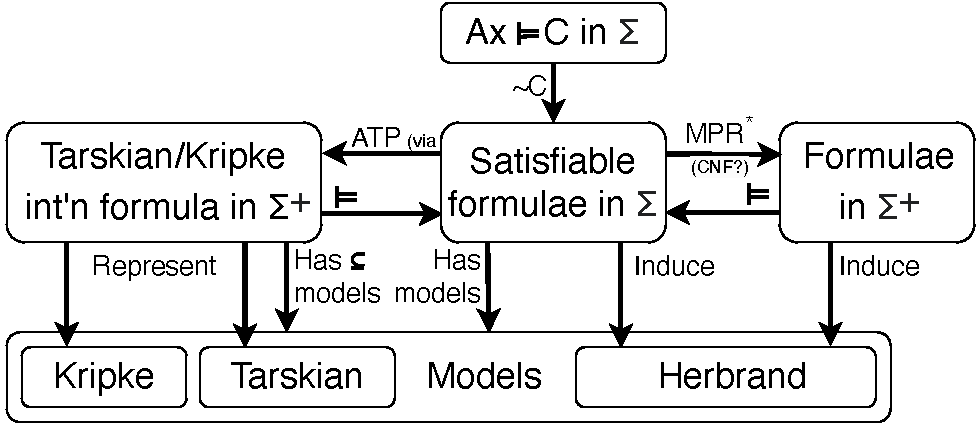
\includegraphics[width=0.75\textwidth]{ModelLandscape.pdf}
\caption{The Landscape of Tarskian Model Building}
\label{ModelLandscape}
\end{figure}

%--------------------------------------------------------------------------------------------------
\section{The New Format for Tarskian Interpretations}
\label{NewTarskian}

As noted in Section~\ref{Introduction}, a TPTP format for interpretations with finite domains 
has previously been defined, and was been adopted by some ATP systems.

The new format uses interpretation-formulae.
Examples of single {\sf D+M} interpretation-formulae are in Appendices~\ref{FOF_Finite.s}, 
\ref{TFF_Finite.s}, \ref{TFF_Integer.s}, \ref{TFF_Peano.s} and~\ref{THF_Finite.s}, illustrating 
the components described next. 
{\sf D+M} interpretations split over multiple interpretation-formulae, as in 
Appendices~\ref{FOF_Finite_Medium.s}, \ref{FOF_Finite_Fine.s}, \ref{TFF_Finite_Medium.s}, 
\ref{TFF_Finite_Fine.s}, and~\ref{THF_Finite_Medium.s} are explained in 
Section~\ref{NewTarskianSplit}.
{\sf D+M} interpretations that are compacted using quantification, as in \ref{TFF_Finite_Compact.s}
and~\ref{THF_Finite_Compact.s} are explained in Section~\ref{NewTarskianCompact}.
Examples of interpretation-formulae that induce Herbrand interpretations, as in 
Appendices~\ref{FOF_Finite_Medium.s}, \ref{FOF_Finite_Fine.s}, \ref{TFF_Finite_Medium.s},
\ref{TFF_Finite_Fine.s}, and~\ref{THF_Finite_Medium.s} are explained in
Section~\ref{NewHerbrand}.
ZZZZZZZZZ

A single interpretation-formula is a conjunction of components:
\begin{packed_itemize}
\item Domain specifications for each of the types in the problem formulae.
\item Interpretation of the function symbols, as equalities whose left-hand sides are formed from 
      symbols applied to domain elements, and whose right-hand sides are domain elements.
\item Interpretation of the predicate symbols, as literals formed from symbols applied
      to domain elements; positive literals are {\em true} and negative literals are {\em false}.
\end{packed_itemize}

Note that function and predicate symbols are interpreted by directly applying them to domain
elements, rather than the traditional presentation of interpretation that introduces a new
interpretation function for each function/predicate symbol \cite[p.999]{Gal15}.
This slight-of-hand simplifies the representation of interpretations, and makes interpretation
of new formulae by ATP more tractable.
The explanations and examples that follow will convince you of that!

%--------------------------------------------------------------------------------------------------
\subsection{Untyped FOF {\sf D+M} Interpretations}
\label{NewTarskianFOF}

For FOF interpretations domain elements are new ground terms, and their distinctness must be 
specified either with pairwise inequalities or with the {\tt \$distinct} predicate.
As terms and domain elements are untyped (or, if you will, of type {\tt \$i}), the interpretation
of symbols can apply the symbols directly to the domain elements; this is not the case for
TFF and TXF, as is explained next.
Appendix~\ref{FOF_Finite.s} shows a FOF interpretation-formula with a finite domain -- it is a 
countermodel for the problem in Appendix~\ref{FOF_Finite.p}.
A convenient way to make the domain elements distinct is to use {\tt "distinct object"} constants, 
which are known to be distinct (and often not used in problems, which makes them easy to identify 
as domain elements).
Appendix~\ref{FOF_Finite.s} uses {\tt "distinct object"}s.
Appendix~\ref{FOF_Finite.s.p} shows the verification problem for the interpretation.

%--------------------------------------------------------------------------------------------------
\subsection{Typed TFF and THF {\sf D+M} Interpretations}
\label{NewTarskianTFFTHF}

For TFF and TXF interpretation-formulae, each type of the problem has a domain, which can be of 
a new type.
If the problem type is different from the domain type then function and predicate symbols from 
the problem cannot be directly applied to domain elements of the type that corresponds to the type
of the argument position.
To resolve this {\em type-promotion} bijection are used to ``convert'' domain elements to terms 
of the corresponding type, thus keeping the interpretation formula well-typed -- See
Appendix~\ref{TFF_Finite.s} for examples.
The interpretation formula is preceded by the necessary type declarations:
\begin{packed_itemize}
\item The types in the problem (except defined types, e.g., {\smalltt{\$int}}).
\item The types of the domains (except defined types).
\item The types of type-promotion functions.
\item The types of the domain elements.
\end{packed_itemize}
Then, (following along in Appendices~\ref{TFF_Finite.s}, \ref{TFF_Integer.s}, and~\ref{TFF_Peano.s} 
might help here) each domain is a conjunction of:
\begin{packed_itemize}
\item The domain for each problem type, as a formula that makes the type-promotion function a 
      surjection (unless it is unnecessary because the domain type is defined and is the same as 
      the problem type, e.g., both are {\smalltt{\$int}}), e.g., in 
      Appendix~\ref{TFF_Finite.s}~\ldots\\
      \hspace*{0.5cm}\smalltt{! [C: cat] : ? [DC: d\_cat] : C = d2cat(DC)}
\item The elements of each domain (unless implicit from their defined type, as in
      Appendix~\ref{TFF_Integer.s}). 
      If the domain is finite this is a universally quantified disjunction of equalities whose 
      right-hand sides are the terms, e.g., in Appendix~\ref{TFF_Finite.s}~\ldots\\
      \hspace*{0.5cm}\smalltt{! [DC: d\_cat]: ( DC = d\_garfield | DC = d\_arlene | DC = d\_nermal )}\\
      If the domain is infinite this is an existentially quantified formula that captures an 
      infinite disjunction of equalities, e.g., in Appendix~\ref{TFF_Peano.s}~\ldots\\
      \hspace*{0.5cm}\smalltt{! [I: peano] : ( I = zero | ? [P: peano] : I = s(P) )}
\item Specification of the distinctness of the domain elements (unless implicit from their
      defined type);
\item A formula making the type-promotion function an injection,
      % (unless the type of the domain is the same as the type in the formula), 
      which together with the surjectivity makes it a bijection.
\end{packed_itemize}
The interpretation of symbols applies the corresponding type-promotion function to each domain
element argument so that that signatures of the symbols are respected.

\begin{packed_itemize}
\item Appendix~\ref{TFF_Finite.s} shows a TF0 interpretation-formula with finite domains -- it is a 
      countermodel for the problem in Appendix~\ref{TFF_Finite.p}.
      The comments show which parts of the formula specify what aspects of the interpretation.
      Appendix~\ref{TFF_Finite.s.p} shows the verification problem for the interpretation.
\item Appendix~\ref{TFF_Integer.s} shows a TF0 interpretation-formula with an integer domain -- it 
      is a model for the problem in Appendix~\ref{TFF_Infinite.p}.
      Note that $\bullet$~the defined type {\smalltt{\$int}} is the domain type for the formula 
      type {\smalltt{person}}, so that there is no specification of the domain elements and their 
      distinctness; $\bullet$~universal quantification is used for the interpretation of function 
      and predicate symbols for an infinite number of argument tuples; $\bullet$~the 
      interpretation of function and predicate symbols is not given for argument tuples with 
      negative integers, i.e., this is an example of a partial interpretation.
      Appendix~\ref{TFF_Integer.s.p} shows the verification problem for the interpretation.
\item Appendix~\ref{TFF_Peano.s} shows a TF0 interpretation-formula with an infinite term domain 
      -- it is a model for the problem in Appendix~\ref{TFF_Infinite.p}.
      Appendix~\ref{TFF_Peano.s.p} shows the verification problem for the interpretation.
\end{packed_itemize}

%--------------------------------------------------------------------------------------------------
\subsection{{\sf D+M} Interpretations Split over Multiple Formulae}
\label{NewTarskianSplit}

The new TPTP format for {\sf D+M} interpretations described thus far puts all the information 
about the interpretation in a single interpretation formula.
In some situations it is useful to separate the various components, e.g., the domains could be
separated from the symbol mappings.
The new TPTP format for {\sf D+M} interpretations offers separation in a flexible way, at medium
and fine grained levels, using annotated formula subroles.

At the medium grained level the {\tt interpretation} role can be extended withe the subroles
{\tt domain} and {\tt mapping}.
Two (or more) interpretation formulae are used, each containing the corresponding parts of the 
interpretation.
Appendices~\ref{FOF_Finite_Medium.s} and \ref{TFF_Finite_Medium.s} show examples.
Note that each role and role-subrole pair can be used multiple times according to need, e.g.,
in Appendix~\ref{FOF_Finite_Medium.s} there are two {\tt interpretation-mapping} annotated
formulae, one for functions and one for predicates.

At the fine grained level the interpretation formula can be split into the individual domains
and symbol mappings, with the {\tt domain} and {\tt mapping} subroles given arguments to indicate
which domain or symbol mapping is recorded.
For {\tt domain}s the arguments are the domain from the problem and the domain in the 
interpretation.
For {\tt mapping}s the arguments are the symbol and its domain result type.
Appendices~\ref{FOF_Finite_Fine.s} and \ref{TFF_Finite_Fine.s} show examples.

The medium and fine grained splitting can be mixed, as is done in 
Appendix~\ref{THF_Finite_Medium.s}.

%--------------------------------------------------------------------------------------------------
\subsection{{\sf D+M} Interpretations Compacted using Quantification}
\label{NewTarskianCompact}

In the context of using theorem proving to evaluate formulae wrt an interpretation represented
by a interpretation formula, it is possible to use the full logical language in the interpretation 
formula.
This enable some comapcting of the interpretation.
Appendices~\ref{TFF_Finite_Compact.s} and \ref{THF_Finite_Compact.s} show examples.
In Appendix~\ref{TFF_Finite_Compact.s} note how universal quantification is used to map
{\tt loves} to {\tt d\_garfield} for all {\tt d\_cats}~\ldots \\
\hspace*{0.5cm}\smalltt{! [DC: d\_cat] : ( loves(d2cat(DC)) = d2cat(d\_garfield) )} \\
and in Appendix~\ref{THF_Finite_Compact.s} universal quantification is used to say that for all
functions of type {\tt beverage > syrup} and all {\tt syrups} applying the function to
{\tt d\_coffee} and the syrup results in {\tt d\_coffee}~\ldots \\
\hspace*{0.5cm}\smalltt{! [F: beverage > syrup > beverage,S: syrup] :} \\
\hspace*{1.0cm}\smalltt{( ( F @ ( d2beverage @ d\_coffee ) @ ( d2syrup @ S ) )} \\
\hspace*{1.0cm}\smalltt{= ( d2beverage @ d\_coffee ) )}

%--------------------------------------------------------------------------------------------------
\section{The New Format for Kripke Interpretations}
\label{NewKripke}
 
The new format uses an {\em interpretation formula}. 
Examples of single interpretation formulae are in 
Appendices~\ref{NTF_Finite-Finite-Global.s}~and~\ref{NTF_Finite-Finite-Local.s}, 
illustrating the components described next. 
Interpretations split over multiple interpretation formulae, as in 
Appendices~\ref{NTF_Finite-Finite-Global_Medium.s}, \ref{NTF_Finite-Finite-Global_Fine.s}, 
and~\ref{NTF_Finite-Finite-Global_Compact.s}, are explained in Section~\ref{NewKripkeSplit}.

%--------------------------------------------------------------------------------------------------
%% \section{Model Verification}
%% \label{Verification}
%% 
%% ATP systems are complex pieces of software, implementing complex calculi, with the end goal
%% being a sound implementation of a sound inference system whose output correctly corroborates the
%% result obtained.
%% The reality is that the complexity leads to incorrectness, and as such verification of ATP systems'
%% outputs is necessary. 
%% For theorem proving this means verifying the proof output \cite{Sut06}, and for model finding 
%% this means verifying the model output.
%% In the context of this work the model verification applies to the type declarations and 
%% the interpretation formula that represent the model found by the ATP system, and
%% has (at least) the following aspects:
%% \begin{packed_enumerate}
%% \item Are the type declarations and interpretation formula syntactically well-formed 
%%       and semantically well-typed?
%% \item Is the interpretation formula satisfiable?
%% \item Does the interpretation formula correctly represent the interpretation found by the 
%%       ATP system?
%% \item Is the interpretation represented by the interpretation formula a model for the given 
%%       formulae?
%% \end{packed_enumerate}
%% \noindent
%% These questions are answered as follows:
%% \begin{enumerate}
%% \item This can be confirmed using standard parsing and type checking tools, e.g., \cite{VS06,HR15}.
%% \item This can be empirically confirmed using a trusted model finder (in the same way the GDV 
%%       derivation verifier \cite{Sut06} uses the Otter system \cite{McC03-Otter} as a trusted 
%%       theorem prover).
%%       Confirming that the interpretation formula is satisfiable is almost certainly much 
%%       easier than finding the model itself, so the system used to check the satisfiability can 
%%       be weaker and more trusted than the system that found the model.
%% \item This cannot be confirmed, as that representation is internal to the ATP system that found
%%       the model.
%% \item In this work a ``semantic'' approach is taken, in which the problem formulae $\Phi$ are 
%%       proved from the interpretation formulae $\varphi$ using a trusted theorem prover. 
%%       $\varphi$ are given as axioms, and $\Phi$ as the conjecture to be proved.
%%       The soundness of this approach is provided by showing that if $\Phi$ can be proved from 
%%       $\varphi$ then the interpretation $I$ represented by $\varphi$ is a model of $\Phi$.
%%       This is shown for finite FOF interpretations in \cite{SS+23-LPAR}, and that theorem lifts 
%%       (we believe) naturally to TFF, and THF, but is technically complicated due to the 
%%       introduction of types and type promotion functions. 
%%       The extension to infinite domains is quite simple after that.
%% \end{enumerate}
      
%--------------------------------------------------------------------------------------------------
\section{Conclusion}
\label{Conclusion}

This paper 

This work is being extended 

%--------------------------------------------------------------------------------------------------
\bibliographystyle{plain}
\bibliography{Bibliography.bib}
%--------------------------------------------------------------------------------------------------
\newpage
\appendix

All these listings are available from
\href{https://github.com/GeoffsPapers/InterpretationFormat}{github.com/GeoffsPapers/InterpretationFormat}.

\section{FOF}
\label{FOF}

\subsection{FOF Problem with a Finite Countermodel}
\label{FOF_Finite.p}
\begin{small}
\verbatiminput{FOF_Finite.p}
\end{small}

\newpage
\subsection{FOF Finite Model for \ref{FOF_Finite.p}, Coarse Grained}
\label{FOF_Finite.s}
\begin{small}
\verbatiminput{FOF_Finite.s}
\end{small}

\newpage
\subsection{FOF Verification Problem for \ref{FOF_Finite.p} and \ref{FOF_Finite.s}}
\label{FOF_Finite.s.p}
\begin{small}
\verbatiminput{FOF_Finite.s.p}
\end{small}

\newpage
\subsection{FOF Finite Model for \ref{FOF_Finite.p}, Medium Grained}
\label{FOF_Finite_Medium.s}
\begin{small}
\verbatiminput{FOF_Finite_Medium.s}
\end{small}

\newpage
\subsection{FOF Finite Model for \ref{FOF_Finite.p}, Fine Grained}
\label{FOF_Finite_Fine.s}
\begin{small}
\verbatiminput{FOF_Finite_Fine.s}
\end{small}

%--------------------------------------------------------------------------------------------------
\newpage
\section{TF0, Finite Interpretations}
\label{TF0Finite}

\subsection{TF0 Problem with a Finite Countermodel}
\label{TFF_Finite.p}
\begin{small}
\verbatiminput{TFF_Finite.p}
\end{small}

\newpage
\subsection{TF0 Finite Model for \ref{TFF_Finite.p}, Coarse Grained}
\label{TFF_Finite.s}
\begin{small}
\verbatiminput{TFF_Finite.s}
\end{small}

\newpage
\subsection{TF0 Verification Problem for \ref{TFF_Finite.p}}
\label{TFF_Finite.s.p}
\begin{small}
\verbatiminput{TFF_Finite.s.p}
\end{small}

\newpage
\subsection{TF0 Finite Model for \ref{TFF_Finite.p}, Medium Grained}
\label{TFF_Finite_Medium.s}
\begin{small}
\verbatiminput{TFF_Finite_Medium.s}
\end{small}

\newpage
\subsection{TF0 Finite Model for \ref{TFF_Finite.p}, Fine Grained}
\label{TFF_Finite_Fine.s}
\begin{small}
\verbatiminput{TFF_Finite_Fine.s}
\end{small}

\newpage
\subsection{TF0 Finite Model for \ref{TFF_Finite.p}, Compacted}
\label{TFF_Finite_Compact.s}
\begin{small}
\verbatiminput{TFF_Finite_Compact.s}
\end{small}

%--------------------------------------------------------------------------------------------------
\newpage
\section{TF0, Infinite Interpretations}
\label{TF0Infinite}

\subsection{TF0 Axioms with an Infinite Model}
\label{TFF_Infinite.p}
\begin{small}
\verbatiminput{TFF_Infinite.p}
\end{small}

\newpage
\subsection{TF0 Infinite Model for \ref{TFF_Infinite.p}, Integer Domain}
\label{TFF_Integer.s}
\begin{small}
\verbatiminput{TFF_Integer.s}
\end{small}

\newpage
\subsection{TF0 Infinite Model for \ref{TFF_Infinite.p}, Term Domain}
\label{TFF_Peano.s}
\begin{small}
\verbatiminput{TFF_Peano.s}
\end{small}

\newpage
\subsection{TF0 Verification Problem for \ref{TFF_Infinite.p} and \ref{TFF_Integer.s}}
\label{TFF_Integer.s.p}
\begin{small}
\verbatiminput{TFF_Integer.s.p}
\end{small}

\newpage
\subsection{TF0 Verification Problem for \ref{TFF_Infinite.p} and \ref{TFF_Peano.s}}
\label{TFF_Peano.s.p}
\begin{small}
\verbatiminput{TFF_Peano.s.p}
\end{small}

%--------------------------------------------------------------------------------------------------
\newpage
\section{TH0, Finite Interpretations}
\label{TH0Finite}

\subsection{TH0 Problem with a Finite Countermodel}
\label{THF_Finite.p}
\begin{small}
\verbatiminput{THF_Finite.p}
\end{small}

\newpage
\subsection{TH0 Finite Model for \ref{THF_Finite.p}, Coarse Grained}
\label{THF_Finite.s}
\begin{small}
\verbatiminput{THF_Finite.s}
\end{small}

\newpage
\subsection{TH0 Verification Problem for \ref{THF_Finite.p}}
\label{THF_Finite.s.p}
\begin{small}
\verbatiminput{THF_Finite.s.p}
\end{small}

\newpage
\subsection{TH0 Finite Model for \ref{THF_Finite.p}, Mixed Grained}
\label{THF_Finite_Medium.s}
\begin{small}
\verbatiminput{THF_Finite_Medium.s}
\end{small}

\newpage
\subsection{TH0 Finite Model for \ref{THF_Finite.p}, Compacted}
\label{THF_Finite_Compact.s}
\begin{small}
\verbatiminput{THF_Finite_Compact.s}
\end{small}

%--------------------------------------------------------------------------------------------------
\newpage
\section{NXF with Global Axioms, \\
         Finite Worlds with Finite Interpretations}
\label{NXFGlobal}

\subsection{NTF Problem with Global Axioms, \\ with a Finite-Finite Countermodel}
\label{NTF_Finite-Finite-Global.p}
\begin{small}
\verbatiminput{NTF_Finite-Finite-Global.p}
\end{small}

\newpage
\subsection{TXF Finite-Finite Model for \ref{NTF_Finite-Finite-Global.p}}
\label{NTF_Finite-Finite-Global.s}
\begin{small}
\verbatiminput{NTF_Finite-Finite-Global.s}
\end{small}

\newpage
\subsection{TXF Finite-Finite Model for \ref{NTF_Finite-Finite-Global.p}, Compacted}
\label{NTF_Finite-Finite-Global_Compact.s}
\begin{small}
\verbatiminput{NTF_Finite-Finite-Global_Compact.s}
\end{small}

\newpage
\subsection{Verification Problem for \ref{NTF_Finite-Finite-Global.p} and 
\ref{NTF_Finite-Finite-Global.s}/\ref{NTF_Finite-Finite-Global_Medium.s}/\ref{NTF_Finite-Finite-Global_Fine.s}}
\label{NTF_Finite-Finite-Global.s.p}
\begin{small}
\verbatiminput{NTF_Finite-Finite-Global.s.p}
\end{small}

\newpage
\subsection{TXF Finite-Finite Model for \ref{NTF_Finite-Finite-Global.p}, Medium Grained}
\label{NTF_Finite-Finite-Global_Medium.s}
\begin{small}
\verbatiminput{NTF_Finite-Finite-Global_Medium.s}
\end{small}

\newpage
\subsection{TXF Finite-Finite Model for \ref{NTF_Finite-Finite-Global.p}, Fine Grained}
\label{NTF_Finite-Finite-Global_Fine.s}
\begin{small}
\verbatiminput{NTF_Finite-Finite-Global_Fine.s}
\end{small}

%--------------------------------------------------------------------------------------------------
\newpage
\section{NXF with Global and Local Axioms, \\
         Finite Worlds with Finite Interpretations}
\label{NXFLocal}

\subsection{NTF Problem with Global and Local Axioms, \\
            with a Finite-Finite Countermodel}
\label{NTF_Finite-Finite-Local.p}
\begin{small}
\verbatiminput{NTF_Finite-Finite-Local.p}
\end{small}

\newpage
\subsection{TXF Finite-Finite Model for \ref{NTF_Finite-Finite-Local.p}}
\label{NTF_Finite-Finite-Local.s}
\begin{small}
\verbatiminput{NTF_Finite-Finite-Local.s}
\end{small}

\newpage
\subsection{Verification Problem for \ref{NTF_Finite-Finite-Local.p} and
\ref{NTF_Finite-Finite-Local.s}}
\label{NTF_Finite-Finite-Local.s.p}
\begin{small}
\verbatiminput{NTF_Finite-Finite-Local.s.p}
\end{small}

%--------------------------------------------------------------------------------------------------
\end{document}
%--------------------------------------------------------------------------------------------------
